%% The UnionLabs Agent — COLUMN variant. Three layers: the cloud, the agent as
%% middleware on every edge node, and what it manages beneath — the experiment
%% container and the physical devices it selectively exposes into it.
\documentclass[tikz,border=4pt]{standalone}
\usepackage{xcolor}
%% Shared look for the UnionLabs system figures. \input by each fig-*.tex so a
%% colour or a corner radius is changed in one place.
\usetikzlibrary{positioning,arrows.meta,fit,backgrounds,calc}

\definecolor{uCode}{HTML}{1F6F5C}     % the experimenter's own code
\definecolor{uApi}{HTML}{6B4BA8}      % the contract / ARQ layer
\definecolor{uPhy}{HTML}{2E5E9E}      % transports / DSP
\definecolor{uRadio}{HTML}{B4700F}    % hardware
\definecolor{uShare}{HTML}{8A2E4D}    % the shared workspace

\tikzset{
  blk/.style={draw, rounded corners=2pt, align=center, font=\small,
              minimum height=8mm, inner sep=3pt, fill=black!2},
  code/.style={blk, draw=uCode, thick, fill=uCode!6},
  api/.style={blk, draw=uApi, very thick, fill=uApi!7},
  phy/.style={blk, draw=uPhy, thick, fill=uPhy!6},
  radio/.style={blk, draw=uRadio, thick, fill=uRadio!8},
  share/.style={blk, draw=uShare, thick, fill=uShare!6},
  stage/.style={blk, minimum height=9.5mm, font=\scriptsize, text width=16mm,
                inner sep=2pt},
  flow/.style={-{Latex[length=2mm]}, thick},
  back/.style={-{Latex[length=2mm]}, thick, densely dashed},
  % labels that sit ON an arrow: opaque, so the line never strikes the text
  onarrow/.style={font=\scriptsize\itshape, fill=white, inner sep=1.5pt},
  lbl/.style={font=\scriptsize\itshape, inner sep=1pt},
  note/.style={font=\scriptsize, align=left, inner sep=1pt},
  legend/.style={draw, minimum width=3mm, minimum height=3mm, inner sep=0pt},
}
\newcommand{\mono}[1]{{\ttfamily\footnotesize #1}}
\newcommand{\monos}[1]{{\ttfamily\scriptsize #1}}

\begin{document}
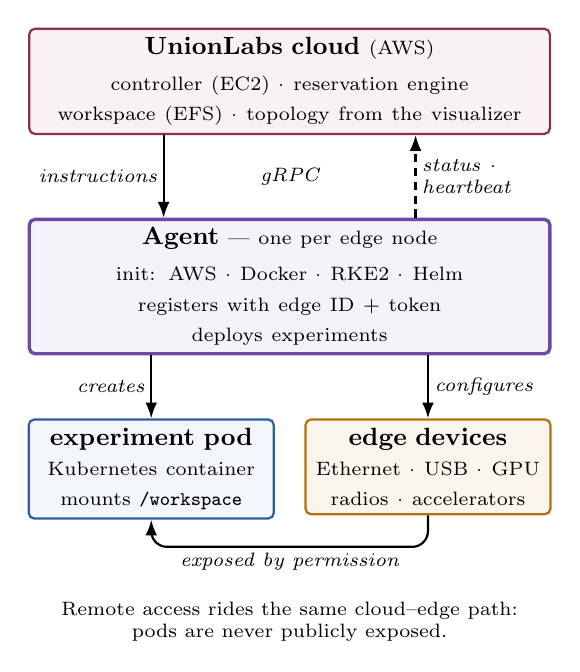
\begin{tikzpicture}[x=1mm, y=1mm,
  duplex/.style={{Latex[length=2mm]}-{Latex[length=2mm]}, thick}]

%% ── the cloud ────────────────────────────────────────────────────────────
\node[share, text width=64mm] (cloud) at (0,0)
  {\textbf{UnionLabs cloud} {\scriptsize (AWS)}\\[2pt]
   {\scriptsize controller (EC2) · reservation engine}\\
   {\scriptsize workspace (EFS) · topology from the visualizer}};

%% ── the agent ────────────────────────────────────────────────────────────
\node[api, text width=64mm, below=10.5mm of cloud] (agent)
  {\textbf{Agent} {\scriptsize --- one per edge node}\\[2pt]
   {\scriptsize init: AWS · Docker · RKE2 · Helm}\\
   {\scriptsize registers with edge ID + token}\\
   {\scriptsize deploys experiments}};

%% two channels of one gRPC session, drawn inside the boxes' span so the
%% figure is exactly as wide as the windows
\draw[flow] ([xshift=-16mm]cloud.south) --
  node[onarrow, left=0.5pt] {instructions} ([xshift=-16mm]agent.north);
\draw[back] ([xshift=16mm]agent.north) --
  node[onarrow, right=0.5pt, align=left] {status ·\\heartbeat}
  ([xshift=16mm]cloud.south);
\node[onarrow] at ($(cloud.south)!0.5!(agent.north)$) {gRPC};

%% ── what it manages on the node ──────────────────────────────────────────
\node[phy, text width=29mm, below=8mm of agent.south west, anchor=north west] (pod)
  {\textbf{experiment pod}\\{\scriptsize Kubernetes container}\\
   {\scriptsize mounts \monos{/workspace}}};
\node[radio, text width=29mm, below=8mm of agent.south east, anchor=north east] (dev)
  {\textbf{edge devices}\\{\scriptsize Ethernet · USB · GPU}\\
   {\scriptsize radios · accelerators}};

\draw[flow] (agent.south -| pod) -- node[onarrow, left=0.5pt] {creates} (pod.north);
\draw[flow] (agent.south -| dev) -- node[onarrow, right=0.5pt] {configures} (dev.north);
\draw[flow, rounded corners=2mm] (dev.south) -- ++(0,-4)
  -| node[pos=0.25, onarrow, below=0.5pt] {exposed by permission} (pod.south);

%% ── one line, not a paragraph ────────────────────────────────────────────
\node[note, align=center, anchor=north]
  at ([yshift=-3mm]current bounding box.south)
  {Remote access rides the same cloud--edge path:\\
   pods are never publicly exposed.};

\end{tikzpicture}
\end{document}
